\chapter[Results and future developments]{Results and future developments}

\section[Measurements summary]{Measurements summary}

\subsection[Input power levels]{Input power levels}

A number of measurements have been collected during 2016. Figure \ref{g_IP} shows the relation between the average gradient and the input power in the accelerating structure. The measurement points have been selected to allow the comparison between the different running conditions, as outlined in Chap. \ref{chap:motivation}, and are summarised in Table \ref{run_pwr}.

\begin{table}
  \centering
    \begin{tabular}{ c l }
    \hline
    \hline
    Run type		&	Input power (MW)		\\
    \hline
    unloaded 		&	43.3, 41, 38 and 24.6	\\
    loaded			&	43.3, 41 and 38			\\
    anti-loaded		&	6.5					\\
    \hline
    \hline
    \end{tabular}
\caption{Input power levels of measurements in 2016.}
\label{run_pwr}
\end{table}

The measurements at different input power level have not been taken in a precise order, anyway it has been tried to keep long measurement periods as much as possible at the same input power. 
The choice is normally complicated by the fact that the Xbox was not able to provide the maximum RF power level during the year, mainly because of technical problems. The order of the runs at constant input power is reported in Fig. \ref{BDR ALL, in appendix ???}.


\subsubsection{Comparison of loaded and unloaded runs at same average gradient}

For the CLIC test purpose,  carry out a measurement at 100 MV/m average gradient comparing loaded and unloaded runs the would be the most interesting measurement possible. In order to perform it, the input power has to raised from 43.3 MW in the unloaded case to 67.5 MW in the loaded case. 

Unfortunately it was clear from the beginning that reaching 67.5 MW of input power was not possible because the waveguides that deliver the power from the pulse compressor to the structure under test are not conditioned for such high power flux.

Because of this limitation, the choice comes down to perform measurements at the same input power and compare the results. 

During a period of technical problems, it has been anyway collected an unloaded measurement at 24.6 MW of input power, in order to compare it with the correspondent average gradient in the loaded case at 43.3 MW of input power. 

but not enough data ....


\subsubsection{Comparison of loaded and unloaded conditions at same input power}



\subsubsection{Study of the antiloaded runs}



\begin{figure}[h]
\centering 
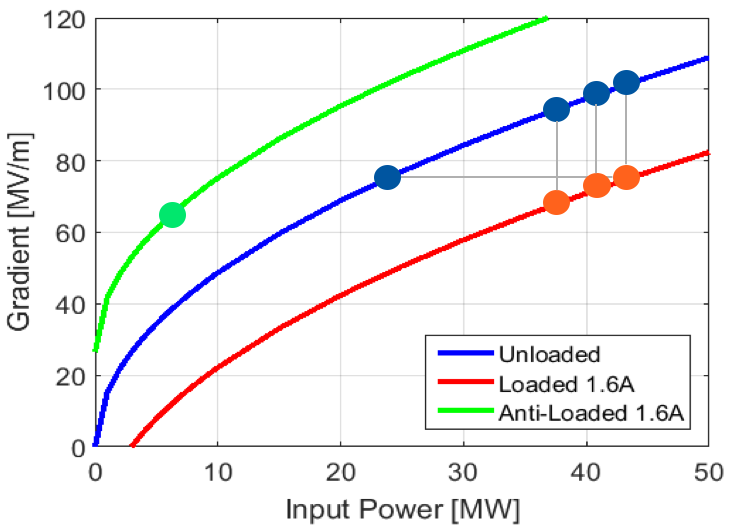
\includegraphics[scale=0.7]{pictures/grad_vs_inPow.png}
\caption{Average gradient as function of the input power in different running conditions. See text for details on the measurement points. }
\label{g_IP}
\end{figure}


\subsection[Beam pulse parameters]{Beam pulse parameters}

As mentioned in the motivation of the experiment, the goal is to understand the effect of the beam on the breakdown rate. The beam parameters have been therefore selected in order to enhance the effect of the beam, rather than try to simulate the CLIC operation. This materialises in:
\begin{itemize}
\item Higher beam current than CLIC: 1.6 A instead of 1.2 A.
\item Longer beam pulse: the beam is lasting during all the compressed RF pulse, for 250 ns, instead of last just during the flat-top of the CLIC pulse (see Sec. \ref{sec:PCtune}).
\end{itemize}




\section[Results]{Results}

\subsection[Breakdown distribution]{Breakdown distribution}



\subsection[Beam induced RF]{Beam induced RF}

Measurements at different input power level have been carried out during 2016. 




\section[Further developments]{Further developments}


RF:
- TWT already eliminated (no spikes anymore)
- I suggest to switch the pulse compressor to a SLED-II type, which is more stable, avoiding all the tuning problems we had
- ?


\section{Conclusions}

During the measurement campaign of this year we learnt how to operate and measure the breakdown rate of the structure with and without beam.

The beam effect analysis has still to be carried on in detail, in particular have to be understood if when running with beam the conditioning takes place or not. Further investigations on this topic require a stable and extensive beam time, which was not the case of the CTF. The comparison of this data with the ones of a stable long test with beam can suggest that switching condition ripetutamente w/ w/o beam can lead to a higher BDR ...
- as DC tests suggest
- as we cannot see because of the low rep.rate



shown effect on the migration !